\subsection{Elements of Morse theory}
In the article, we study the convergence of Mapper graphs towards Reeb graphs under the assumption that the filter function is a Morse function. Note that this assumption is not restrictive as the set of Morse functions is a dense open subset of $C^{\infty}(\man)$, for $\man$ a compact manifold. The aim of this section is to recall the cylindrical structures of preimages of intervals (under a Morse filter function) around non-critical points. See for instance~\cite{milnor1963morse} for a comprehensive presentation of Morse theory.

%\begin{definition}{Morse function.}\label{def:morse}\\
%    Let $\man$ be a differentiable manifold.
%    A smooth map $f\,:\,\man\rightarrow \mathbb{R}$ is called a Morse function if its critical points are non-degenerate, i.e. the Hessian of $f$ at the points where its gradient vanishes is non-singular.
%\end{definition}

%Note that the notion of vanishing gradient and the rank of the Hessian do not depend on the choice of a chart around the point of interest.
%The following proposition shows that Morse functions defined on compact manifolds are generic, in the sense that any smooth function on a compact manifold can be approximated by a Morse function up to any desired precision. See for example Subsection 5.6. in~\cite{laudenbachtransversalite} for a proof.
%\begin{proposition}\label{prop:morse}
%    Let $\man$ be a compact manifold. The set of Morse functions on $\man$ is a dense open subset of $C^{\infty}(\man)$, the space of smooth real functions defined on $\man$.
%\end{proposition}

%Morse theory focuses on studying the topology of a manifold $\man$ using a Morse function $f$ defined on it.\\
Let $\man$ be a Riemannian manifold. Recall that a smooth map $f\,:\,\man\rightarrow \mathbb{R}$ is called a {\it Morse function} if its critical points are non-degenerate, i.e., the Hessian of $f$ at the points where its gradient vanishes is non-singular.  We first recall the standard Morse Lemma, which describes the behavior of a Morse function in the neighborhood of a critical point.  Let $\critic(f)$ denote the set of critical points of a Morse function $f\,:\,\man\rightarrow \R$ defined on $\man$. We will denote $\Vert\cdot\Vert^2:=\g(\cdot, \cdot)$.

\begin{lemma}{Morse Lemma.}\label{lem:morse}\\
Let $f\,:\,\man\rightarrow \mathbb{R}$ be a Morse function and $c\in\critic(f)$. Then there exists a chart $\varphi\,:\,U\subseteq\man\rightarrow \mathbb{R}^d$ containing $c$ such that for every $p\in U$:
    $$f(p)=f(c)-\sum_{j=1}^ix_j^2+\sum_{j=i+1}^dx_j^2,$$
    where $x=\varphi(p)$ and the integer $i$ depends only on the signature of the Hessian at the critical point $c$.
\end{lemma}

In particular, the Morse Lemma implies that the critical points of a Morse function are isolated, and $\critic(f)$ is finite when $f$ is a Morse function defined on a compact manifold.
%
%Writing the gradient in the chart described in Lemma~\ref{lem:morse} proves that the critical points of a Morse function are isolated. Therefore, we will often use Lemma~\ref{lem:morse} to justify that $\critic(f)$ is finite, when $f$ is a Morse function defined on a compact manifold.\\
Next, we recall a major result that relates the topology of a manifold to the analytic properties of a Morse function defined on it. See Figure \ref{fig:reeb_cylindre} for an illustration.

\begin{lemma}{Gradient flow of a smooth function.}\label{lem:flow}\\
Let $f\,:\,\man\rightarrow \R$ be a smooth function defined on a compact manifold $\man$ and $a,b\in\R$ such that $a<b$.
If $\preim{f}{[a,b]}\cap \critic(f)=\varnothing$,
%does not contain critical points, 
then there exists a diffeomorphism $\psi_{b-a}$ between $\preim{f}{\{a\}}$ and $\preim{f}{\{b\}}$.

\end{lemma}
We provide the proof of this well-known result here, as we will make use of this gradient flow several times later in the article. 
\begin{proof}
Since $\preim{f}{[a,b]}$ does not contain critical points, the following function is well defined:

$$\rho\colon \left \{
\begin{aligned}
\man  &\longrightarrow \R\\
q &\longmapsto \begin{cases}
\frac{1}{\Vert\nabla f(q)\Vert^2}& \text{if } f(q)\in [a,b],\\
0& \text{otherwise.}
\end{cases}
\end{aligned}
\right.,
$$

Now, consider the vector field defined by $X_q=\rho(q)\cdot\nabla f(q)$ and the flow $(\psi_t)_{t\in\R}$ associated to $X_q$. In other words, $\psi_t$ is the solution of the differential equation: 
$$\frac{d\psi_t(p)}{dt}=X_{\psi_t(p)},\,\psi_0(p)=p.$$
For details on the existence and uniqueness of $\psi_t$, see Lemma~$2.4.$ of \cite{milnor1963morse}. The main assumption made is that $X_q$ vanishes outside a compact subset of $\man$, which is true in our case since $\man$ is compact and $\preim{f}{[a,b]}$ is closed. Note that $\forall t\in\R$, $\psi_t$ is a diffeomorphism. Also, $\psi_t\circ\psi_s=\psi_{t+s}$.

Notice that we constructed $\rho$ so that for every $p\in \preim{f}{[a,b]}$, with the notation $q=\psi_t(p)$, we have:
\begin{align*}
\frac{d(f\circ\psi_t)(p)}{dt}&=\g\left(\frac{d\psi_t(p)}{dt},\nabla f(q)\right)\\
&=\g\left(\frac{\nabla f(q)}{\Vert\nabla f(q)\Vert^2},\nabla f(q)\right)\\
&=1.
\end{align*}
Consequently, $f\circ\psi_t(p)\colon t\mapsto t+f(p)$, and therefore $$\psi_{b-a}\left(\preim{f}{\{a\}}\right)= \preim{f}{\{b\}},$$
and 
$$\psi_{a-b}\left(\preim{f}{\{b\}}\right)= \preim{f}{\{a\}}.$$
Finally, $\psi_{b-a}$ is a diffeomorphism between $\preim{f}{\{a\}}$ and $\preim{f}{\{b\}}$.

\end{proof}

This following result is proved implicitly in Theorem 3.1 in~\cite{milnor1963morse}. It is used for example in~\cite{de2016categorified} to show that Reeb graphs are an example of what the authors call {\it constructible spaces}. For the sake of completeness, we give here a full proof. See Figure~\ref{fig:reeb_cylindre}.

\begin{theorem}{Cylindrical shape around non-critical points.}\label{thm:morse}\\
Let $f\,:\,\man\rightarrow \R$ be a Morse function defined on a connected compact Riemannian manifold $\man$. Let also $x\in\man$ such that $x\not\in \critic(f)$, 
%is not a critical value 
and let $v=f(x)$. 
For a small enough $\eps>0$ such that $\preim{f}{[v-\eps,v+\eps]}$ does not contain critical points, the following map is a homeomorphism:
\begin{align*}
\psi\colon \preim{f}{\{v\}}\times[-\eps,\eps] &\longrightarrow \preim{f}{[v-\eps,v+\eps]}  \\
(q,t)&\longmapsto \psi_{t}(q)
\end{align*}
\end{theorem}

\begin{proof}
First, notice that an $\eps>0$ satisfying the assumption of the theorem always exists. By Lemma \ref{lem:morse}, $\critic(f)$ is finite. As such, there exists $\eps>0$ such that $\preim{f}{[v-\eps,v+\eps]}$ contains no critical points. Hence, let $\eps>0$ be such a positive real number. Then, for every $v'\in[v-\eps,v+\eps]$, Lemma~\ref{lem:flow} ensures that $\preim{f}{\{v\}}$ and $\preim{f}{\{v'\}}$ are diffeomorphic, under the map $\psi_{v'-v}$ corresponding to the gradient flow of $f$.\\
Define 
\begin{align*}
\psi\colon \preim{f}{\{v\}}\times[-\eps,\eps] &\longrightarrow \preim{f}{[v-\eps,v+\eps]}  \\
(q,t)&\longmapsto \psi_{t}(q)
\end{align*}

The function $\psi$ is continuous because it is locally Lipschitz: 
\begin{itemize}
    \item for a fixed $q\in \preim{f}{\{v\}}$: $t\mapsto\psi_{t}(q)$ is locally Lipschitz as it is continuously differentiable,
    \item for a fixed $t\in [-\eps,\eps]$: $q\mapsto\psi_{t}(q)$ is locally Lipschitz as it is a diffeomorphism.
\end{itemize}
The inverse of $\psi$ is given by $\psi^{-1}\colon p \longmapsto (\psi_{v-f(p)}(p),f(p)-v)$, which we now prove is continuous. Let $p\in \preim{f}{[v-\eps,v+\eps]}$ and $(p_n)_{n\in\N}$ a sequence in $\preim{f}{[v-\eps,v+\eps]}$ such that $p_n\converge p$.\\
We have:
$$\dis(\psi_{v-f(p)}(p),\psi_{v-f(p_n)}(p_n))\leq \dis(\psi_{v-f(p)}(p),\psi_{v-f(p)}(p_n))+\dis(\psi_{v-f(p)}(p_n),\psi_{v-f(p_n)}(p_n)).$$
Now, as mentioned above, the function $q\mapsto\psi_{v-f(p)}(q)$ is continuous because it is a diffeomorphism. Hence:
$$\dis(\psi_{v-f(p)}(p),\psi_{v-f(p)}(p_n))\converge 0.$$
Moreover,

\begin{align*}
 \dis(\psi_{v-f(p)}(p_n),\psi_{v-f(p_n)}(p_n))&\leq \left|\int_{v-f(p)}^{v-f(p_n)}\left\Vert\frac{d\psi_{u}(p_n)}{du}\right\Vert\,du \right| \\
 &\leq \left|\int_{v-f(p)}^{v-f(p_n)}\frac{1}{\Vert\nabla f(\psi_{u}(p_n))\Vert}\,du \right|.
\end{align*}

As $f$ is smooth and $\preim{f}{[v-\eps,v+\eps]}\cap\critic(f)=\varnothing$, and  denoting:
$$L:=\sup_{q\in \preim{f}{[v-\eps,v+\eps]}}\frac{1}{\Vert\nabla f(q)\Vert},$$
we have $L<\infty$. Therefore,
$$\dis(\psi_{v-f(p)}(p_n),\psi_{v-f(p_n)}(p_n)\leq L\cdot |f(p)-f(p_n)|\converge 0.$$

Finally, we showed that $$\dis(\psi_{v-f(p)}(p),\psi_{v-f(p_n)}(p_n))\converge 0,$$ and thus that $\psi^{-1}$ is continuous.
\end{proof}


\begin{figure}[t]
    \centering
    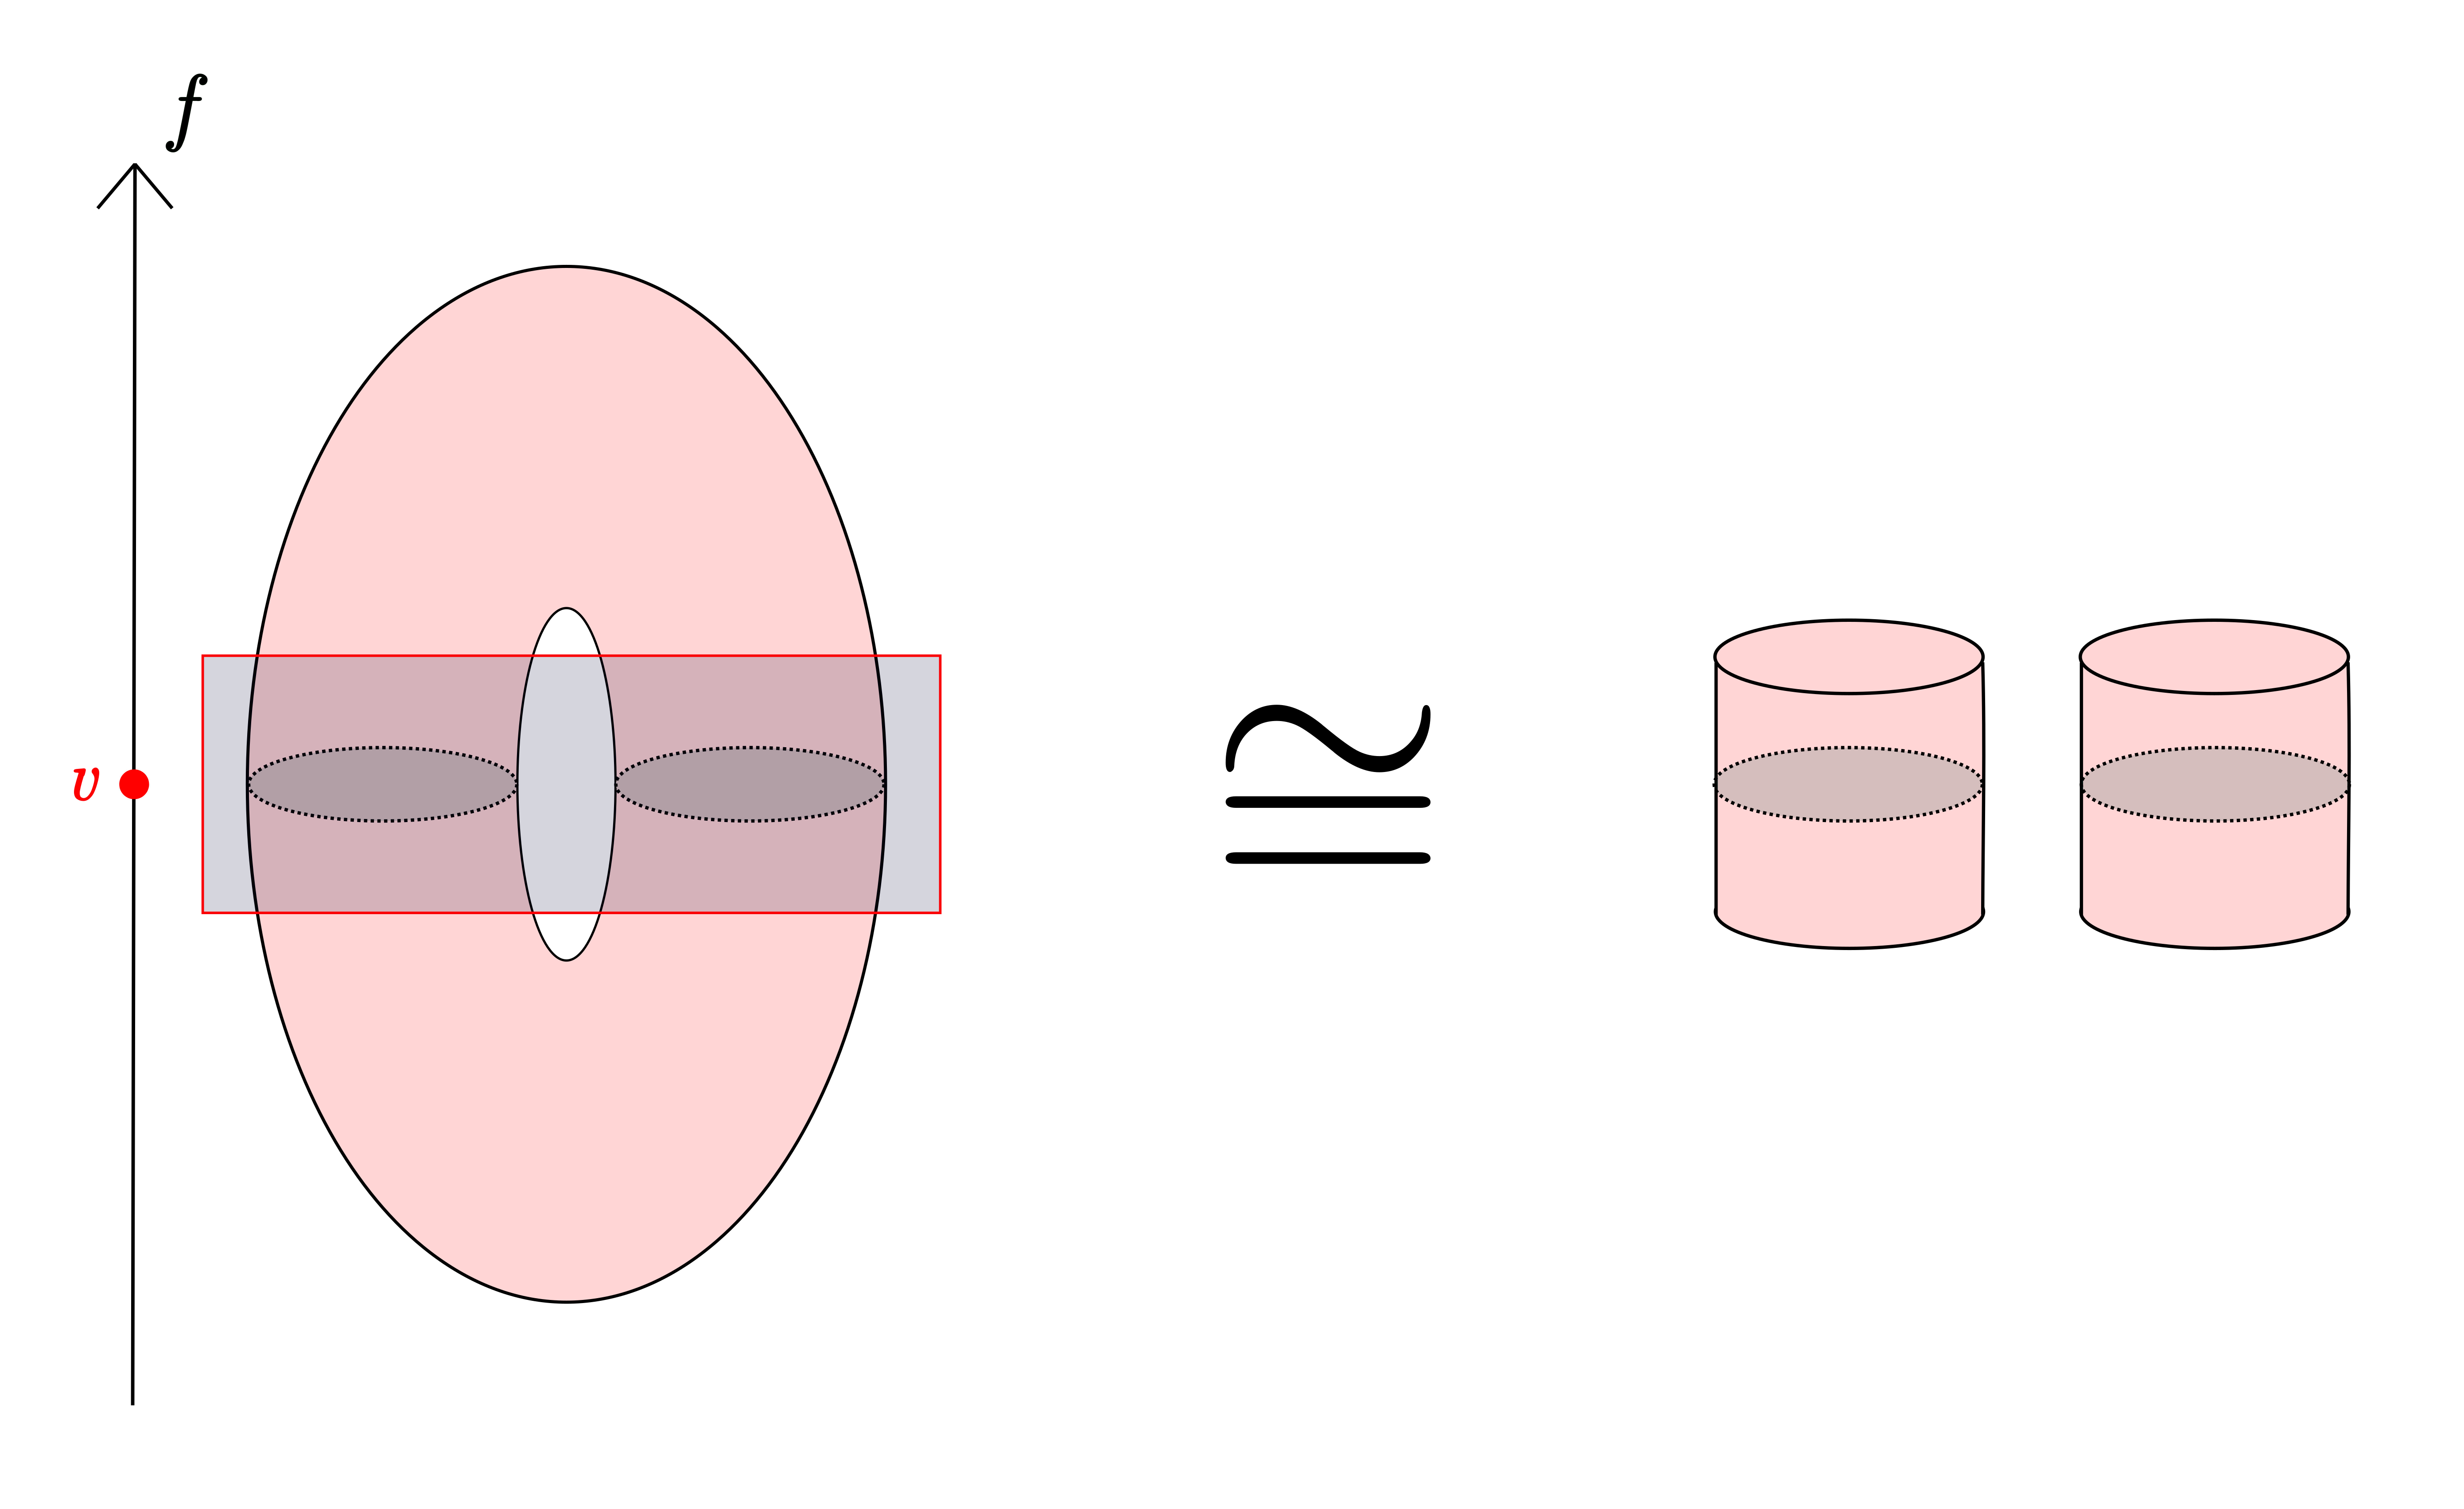
\includegraphics[width=0.7\textwidth]{images/reeb_cylindre.png}
    \caption{\label{fig:reeb_cylindre} Around a non-critical value $v$, the manifold is homeomorphic to a finite collection of cylinders, whose faces are given by the level set $\preim{f}{\{v\}}$.}
\end{figure}

In the context of studying Reeb graphs built on Morse functions, we will use the following Proposition.
\begin{proposition}\label{prop:local_path_con}
Let $f\,:\,\man\rightarrow \R$ be a Morse function defined on a connected compact Riemannian manifold $\man$. The level sets of $f$, $ \preim{f}{\{v\}}$ for $v\in f(\man)$, are locally path connected.
\end{proposition}
\begin{proof}
When $v\in f(\man)$ is not critical, the Implicit Function Theorem (see Theorem 5.8. of~\cite{boothby1986introduction} for example) shows that $\preim{f}{\{v\}}$ is a submanifold of $\man$ and as such is locally path connected.\\
Now, let $v\in f(\man)$ be a critical value. First, $\preim{f}{\{v\}}$ is locally path connected around critical points:\\
Let $c\in\preim{f}{\{v\}}$ be a critical point. By Lemma~\ref{lem:morse}, there exists an open neighborhood $U\subseteq\man$ of $c$ and a chart $\varphi\,:\,U\subseteq\man\rightarrow \mathbb{R}^d$ containing $c$ such that for every $p\in U$:
$$f(p)=f(c)-\sum_{j=1}^ix_j^2+\sum_{j=i+1}^dx_j^2,$$
where $x=\varphi(p)$ and the integer $i$ depends only on the signature of the Hessian at the critical point $c$.\\
Notice that the level set $\preim{f}{\{v\}}$ is given in local coordinates by 
$$\preim{f}{\{v\}}\cap U=\left\{\varphi^{-1}(x):\,\sum_{j=1}^ix_j^2=\sum_{j=i+1}^dx_j^2\right\},$$
and that $\varphi(c)=0$. For every $p\in\preim{f}{\{v\}}\cap U$, the path $\gamma\colon t\mapsto \varphi^{-1}(t\cdot\varphi(p))$ between $c$ and $p$ stays in $\preim{f}{\{v\}}\cap U$. This is because for every $t\in[0,1]$
\begin{align*}
\sum_{j=1}^i\varphi(\gamma(t))_j^2-\sum_{j=i+1}^d\varphi(\gamma(t))_j^2&=t^2\cdot\left(\sum_{j=1}^i\varphi(p)_j^2-\sum_{j=i+1}^d\varphi(p)_j^2\right)\\
&=0.
\end{align*}
Moreover, $\preim{f}{\{v\}}$ is locally path connected away from critical points. The set $\critic(f)$ is finite and hence closed. Therefore, $\man'=\man\setminus\critic(f)$ is an open submanifold of $\man$. Using the Implicit Function Theorem on the restriction of $f$ on $\man'$ as $v$ is no longer a critical value, $\preim{f}{\{v\}}\cap\man'$ is locally path connected.
\end{proof}

Proposition~\ref{prop:local_path_con} has two major applications:
\begin{itemize}
\item When looking at the level sets of a Morse function defined on a compact Riemannian manifold, connectedness and path connectedness are equivalent. Therefore, in what follows, we will use the term \emph{connected} to mean both.
\item The number of connected components of a level set of a  Morse function defined on a compact Riemannian manifold is always finite, as a level set is always compact and locally path connected.
\end{itemize}





















